\section{definition6}
\begin{definition}
\end{definition}
Suppose we have a Riemann sphere $C$ and a diagram $(C,\iota,\xi)$ and a regular cell complex refinement $\overline{(C,\iota,\xi)}$ and a sheaf $\mathfrak{F}$ singular supported on it such that when restricted to a small disk $D\subset C$, the refinement is as following figure where 2 dimensional strata are labeled by tuples

\begin{figure}[H] % Optional: [h] means here, [t] for top, [b] for bottom, [p] for page of floats
    \centering
    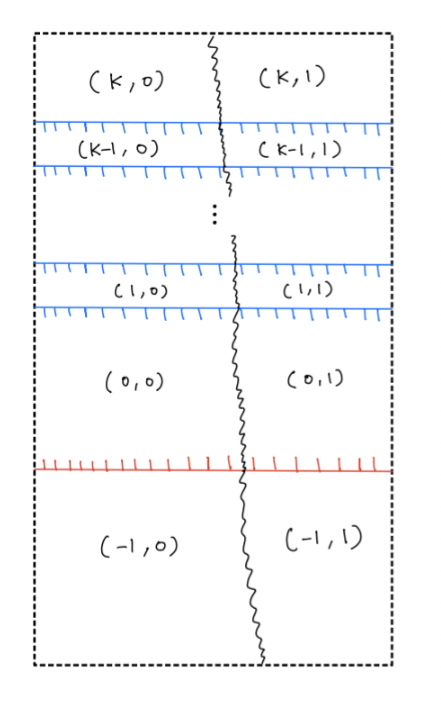
\includegraphics[scale = 0.95]{diagrams/definition6/1.png} % Adjust the width as needed
    \caption{Your caption here}
    \label{fig:your-label}
\end{figure}

Stalks :\\
- $(i,0)$ : $\mathbb{C}^{m+|i|}$\\
- $(i,1)$ : $\mathbb{C}^{m+|i|}$\\

Generization maps\\
- the maps corresponding to the arrow crossing the red strand is $\iota_f$\\
- the maps corresponding to the arrow crossing the blue strand is $\iota_l$\\
- $(i,0)\rightarrow (i,1)$ where $i\geq 0$ : $\tilde{T}_{k+1-i,m+k}$\\
- $(i,0)\rightarrow (i,1)$ where $i=-1$ : $\tilde{T}_{k+1,m+k+1}$\\
\\
where $\tilde{T}_{1,m+k}$ is an isomorphism preserving the flag $\mathbb{C}^m\subset_l \mathbb{C}^{m+1}\subset_l \cdots \subset_l \mathbb{C}^{m+k}$ and $T_{k+1,m+k+2}$ is an isomorphism preserving the flag $\mathbb{C}^m \subset_f \mathbb{C}^{m+1}$.

Now we will define isotopy starting from the above sheaf $\mathfrak{F}$ inductively on the number of blue strands so that the final sheaf $\mathfrak{F}'$ is
\begin{figure}[H] % Optional: [h] means here, [t] for top, [b] for bottom, [p] for page of floats
    \centering
    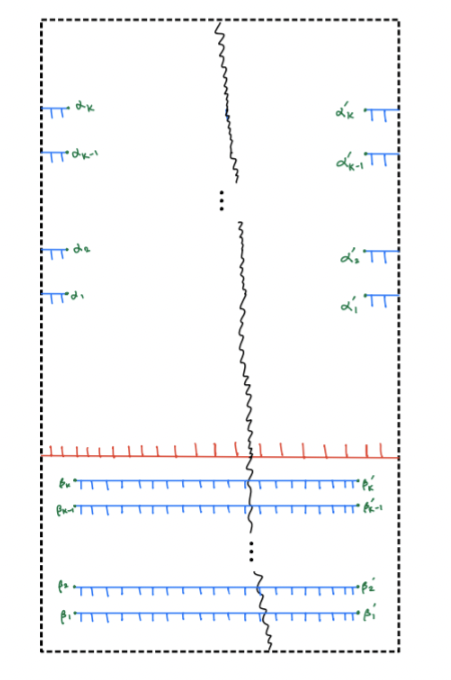
\includegraphics[scale = 0.95]{diagrams/definition6/2.png} % Adjust the width as needed
    \caption{Your caption here}
    \label{fig:your-label}
\end{figure}

In the above diagram, I have intentionally omitted lines connecting
- $\alpha_i$ and $\beta_i$
- $\alpha'_i$ and $\beta'_i$
for $i=1,\cdots,k$ so as not to make diagram too messy. These omitted lines are mutually disjoint and crosses red strand only once.
Let the crossing of the red strand with $\overline{\alpha_i \beta_i}$ be called $c_i$ and $\overline{\alpha'_i \beta'_i}$ be called $c'_i$.
Let's denote the north, east, west, south of the crossing $c_i$($c'_i$ resp.) as $N_i,E_i,W_i,S_i$($N'_i,E'_i,W'_i,S'_i$ resp.).

The final sheaf will be described as follows:

Stalks\\
- $W_i,E'_i$ : $\mathbb{C}^{m+i}$ \\
- $N_i,N'_i$ : $\mathbb{C}^{m+i+1}$ \\
- $S_1,E_1$ : $\mathbb{C}^{m}, \mathbb{C}^{m+1}$\\
- $W'_1,S'_1$ : $\mathbb{C}^{m+1}, \mathbb{C}^m$\\

Generization maps\\ 
- maps crossing blue strands are $\iota_l$\\
- maps crossing red strands are $\iota_f$\\
- maps crossing squiggly lines are\\
	- $E_1\rightarrow W'_1$ : $T' = \tilde{T}_{k+!,m+k+1}$\\
	- $W_k\rightarrow E'_k$ : $T = \tilde{T}_{1,m+k}$\\
	- $N_i \rightarrow N'_i$ : $\tilde{T}_{k-i+1,m+k+1}$\\
	
	
when n=1, (skip this part for now)

Suppose $isotopy_6$ is defined up to the number of blue strands less than $n$. Now we define $isotopy_6$ for the number of blue strands $=n$.

(step1) Apply $isotopy_6$ for the number of blue strands $n-1$ on the disk surrounded by purple dotted line which is well-defined by the induction hypothesis.

\begin{figure}[H] % Optional: [h] means here, [t] for top, [b] for bottom, [p] for page of floats
    \centering
    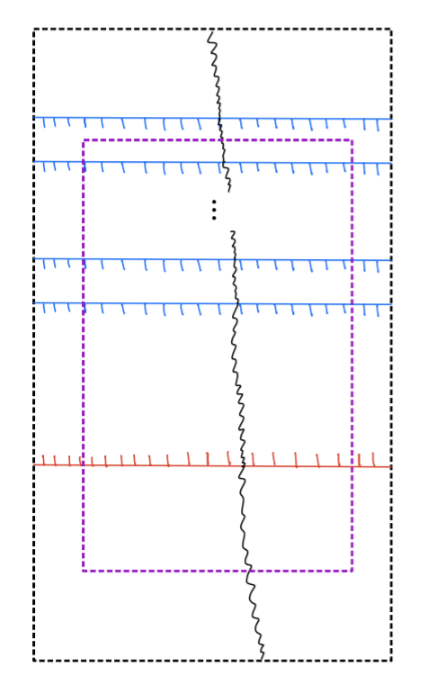
\includegraphics[scale = 0.95]{diagrams/definition6/3.png} % Adjust the width as needed
    \caption{Your caption here}
    \label{fig:your-label}
\end{figure}

we get the following diagram

\begin{figure}[H] % Optional: [h] means here, [t] for top, [b] for bottom, [p] for page of floats
    \centering
    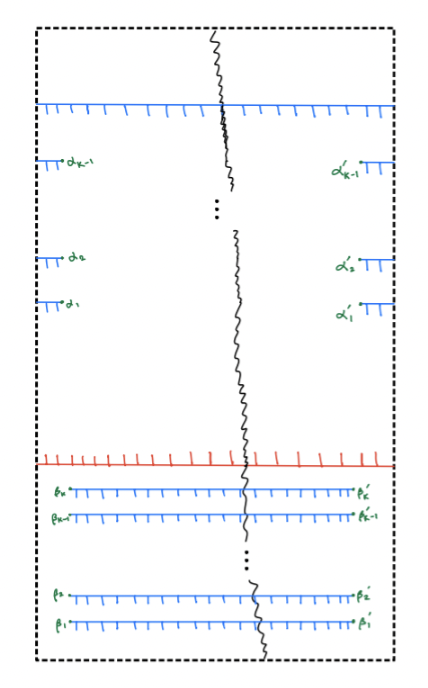
\includegraphics[scale = 0.95]{diagrams/definition6/4.png} % Adjust the width as needed
    \caption{Your caption here}
    \label{fig:your-label}
\end{figure}

(step2) Apply $isotopy_6$ for the number of blue strands $=1$ on the disk surrounded by purple dotted line

\begin{figure}[H] % Optional: [h] means here, [t] for top, [b] for bottom, [p] for page of floats
    \centering
    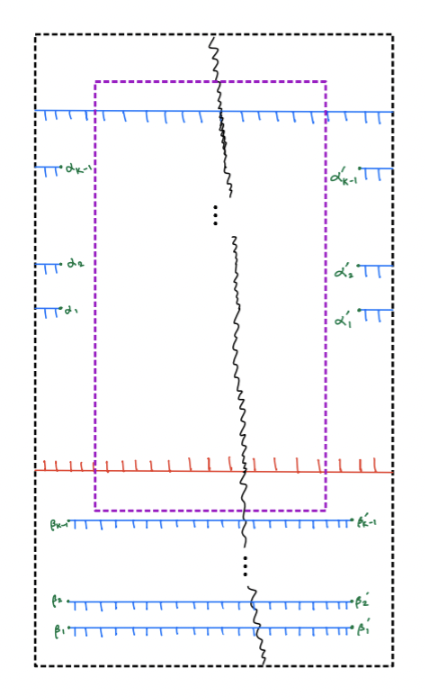
\includegraphics[scale = 0.95]{diagrams/definition6/5.png} % Adjust the width as needed
    \caption{Your caption here}
    \label{fig:your-label}
\end{figure}

we get the final diagram

\begin{figure}[H] % Optional: [h] means here, [t] for top, [b] for bottom, [p] for page of floats
    \centering
    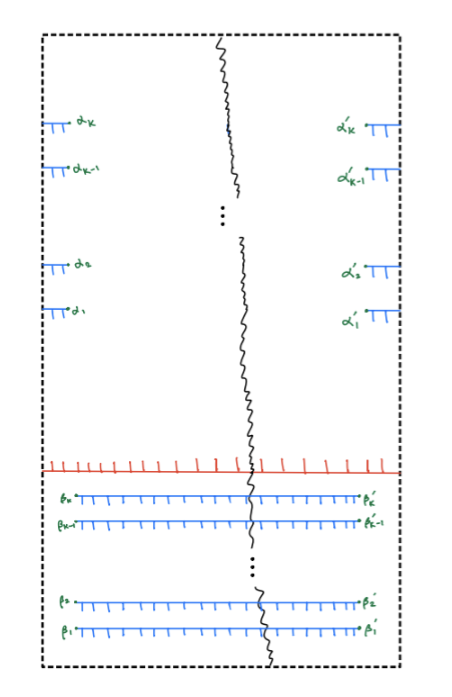
\includegraphics[scale = 0.95]{diagrams/definition6/6.png} % Adjust the width as needed
    \caption{Your caption here}
    \label{fig:your-label}
\end{figure}

with sheaf $\mathfrak{F}$ on it.
(proof)